\documentclass[tikz,border=5mm]{standalone}
\usepackage{tikz}
\usetikzlibrary{arrows.meta,positioning,calc,fit,backgrounds,shapes.geometric,
                decorations.pathmorphing,patterns}
\usepackage{amsmath,amssymb}
\usepackage[T1]{fontenc}
\usepackage{lmodern}

% ── Palette ──────────────────────────────────────────────────────────
\definecolor{csafety}{HTML}{2196F3}
\definecolor{cadv}{HTML}{F44336}
\definecolor{cquery}{HTML}{9E9E9E}
\definecolor{chead}{HTML}{FF9800}
\definecolor{cheadoff}{HTML}{E0E0E0}
\definecolor{ccomply}{HTML}{4CAF50}  % not used here but reserved
\definecolor{crefuse}{HTML}{2196F3}
\definecolor{cflow}{HTML}{7C4DFF}
\definecolor{cbg}{HTML}{FAFAFA}

\begin{document}
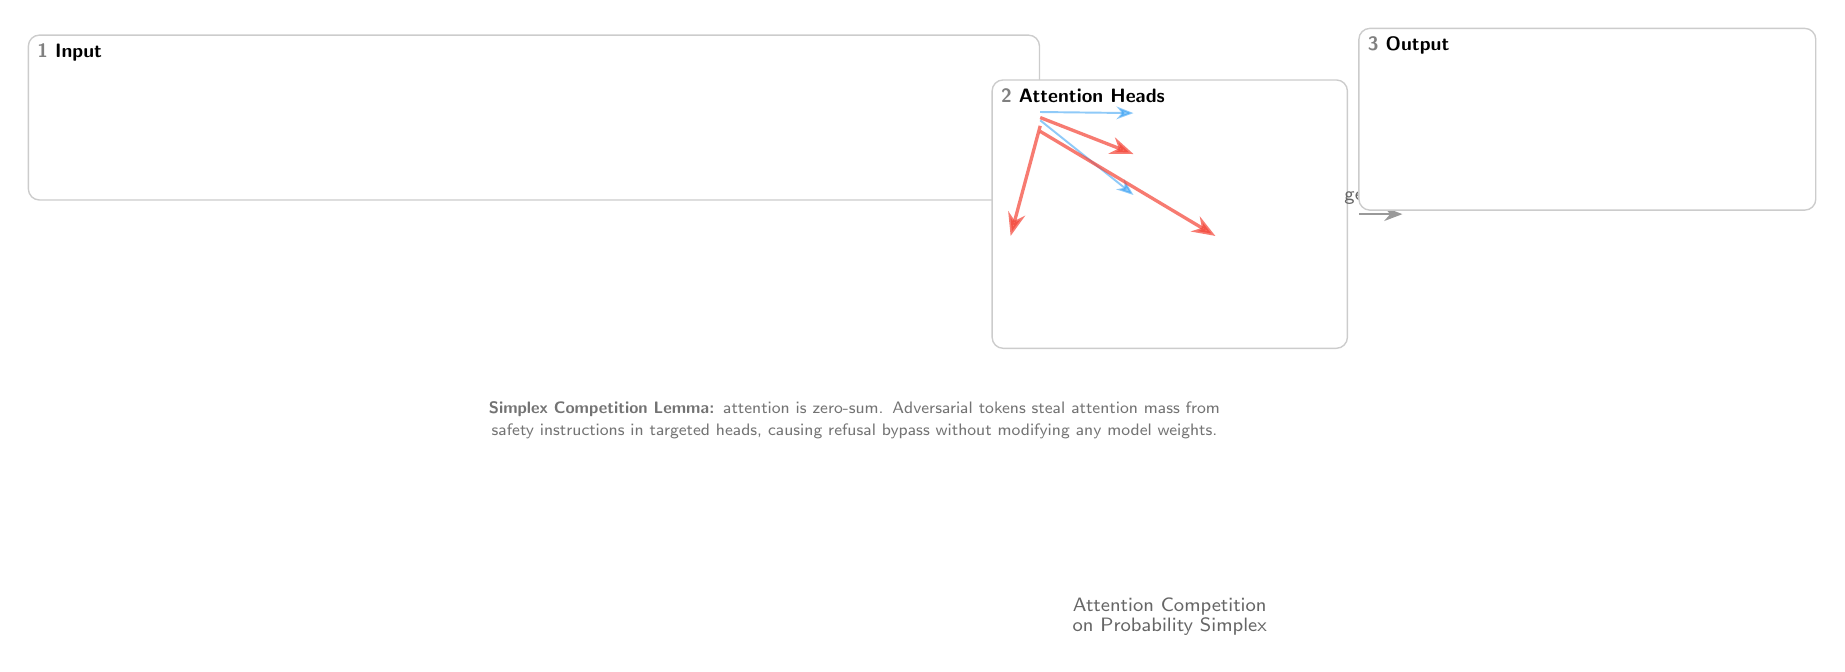
\begin{tikzpicture}[
    >=Stealth,
    font=\sffamily\small,
    token/.style={minimum width=5.6mm, minimum height=5mm, inner sep=0pt,
                  draw=#1, fill=#1!18, line width=0.4pt, rounded corners=1pt},
    stage/.style={draw=black!20, rounded corners=4pt, inner sep=6pt,
                  fill=white, line width=0.5pt},
    annot/.style={font=\sffamily\scriptsize, text=black!60},
    headbox/.style={minimum size=4.2mm, inner sep=0pt, rounded corners=0.5pt,
                    line width=0.35pt},
]

% =====================================================================
% STAGE 1 — Input Construction
% =====================================================================
\begin{scope}[local bounding box=stage1]
  % System prompt tokens
  \foreach \i in {0,...,7} {
    \node[token=csafety] (s\i) at (\i*0.62, 0) {};
  }
  \node[annot, above=1pt of s3.north, anchor=south] {System Prompt};

  % ARA adversarial tokens (dashed border = adversarial)
  \foreach \i in {0,...,4} {
    \node[token=cadv, densely dashed]
      (a\i) at ({8*0.62 + 0.35 + \i*0.62}, 0) {};
  }
  \node[annot, above=1pt of a2.north, anchor=south, text=cadv] {ARA $(k\!=\!5)$};

  % User query tokens
  \foreach \i in {0,...,5} {
    \node[token=cquery] (q\i) at ({8*0.62 + 5*0.62 + 0.7 + \i*0.62}, 0) {};
  }
  \node[annot, above=1pt of q2.north, anchor=south] {User Query};

  % Brace / label underneath
  \node[annot, below=5pt of a2.south, anchor=north] {Input Sequence};
\end{scope}

% Stage 1 box
\node[stage, fit=(stage1), label={[font=\sffamily\scriptsize\bfseries,
      anchor=north west]north west:{\textcolor{black!50}{1}}~Input}] (s1box) {};

% =====================================================================
% Arrow 1→2
% =====================================================================
\draw[->, thick, black!40] ([xshift=4pt]s1box.east) -- ++(0.55,0)
  node[midway, above, annot] {forward};

% =====================================================================
% STAGE 2 — Transformer + Attention Heads
% =====================================================================
\begin{scope}[shift={(12.2,0)}, local bounding box=stage2]
  % Head grid 4×8
  \foreach \r in {0,...,3} {
    \foreach \c in {0,...,7} {
      \pgfmathtruncatemacro{\idx}{\r*8+\c}
      % Mark 5 heads as safety heads
      \ifnum\idx=3  \def\hcol{chead}\else
      \ifnum\idx=11 \def\hcol{chead}\else
      \ifnum\idx=19 \def\hcol{chead}\else
      \ifnum\idx=24 \def\hcol{chead}\else
      \ifnum\idx=29 \def\hcol{chead}\else
                    \def\hcol{cheadoff}\fi\fi\fi\fi\fi
      \node[headbox, draw=\hcol!70, fill=\hcol!35] (h\idx)
        at ({\c*0.52}, {-\r*0.52}) {};
    }
  }

  % Tiny labels on safety heads
  \node[font=\sffamily\fontsize{3.5}{4}\selectfont, text=chead!80]
    at (h3)  {\textbf{0,29}};
  \node[font=\sffamily\fontsize{3.5}{4}\selectfont, text=chead!80]
    at (h11) {\textbf{0,19}};
  \node[font=\sffamily\fontsize{3.5}{4}\selectfont, text=chead!80]
    at (h19) {\textbf{2,0}};
  \node[font=\sffamily\fontsize{3.5}{4}\selectfont, text=chead!80]
    at (h24) {\textbf{2,4}};
  \node[font=\sffamily\fontsize{3.5}{4}\selectfont, text=chead!80]
    at (h29) {\textbf{14,18}};

  % Legend
  \node[headbox, draw=chead!70, fill=chead!35, minimum size=3.2mm]
    (legS) at (0, -2.55) {};
  \node[right=1pt of legS, annot] {Safety head};
  \node[headbox, draw=cheadoff!70, fill=cheadoff!35, minimum size=3.2mm]
    (legN) at (2.1, -2.55) {};
  \node[right=1pt of legN, annot] {Other head};
\end{scope}

% Transformer rounded box
\node[stage, fit=(stage2), label={[font=\sffamily\scriptsize\bfseries,
      anchor=north west]north west:{\textcolor{black!50}{2}}~Attention Heads}]
  (s2box) {};

% ── Attention flow arrows (safety → heads) ──
\draw[->, csafety, line width=0.7pt, opacity=0.5]
  ([yshift=2pt]s1box.east) -- (h3.west);
\draw[->, csafety, line width=0.7pt, opacity=0.5]
  ([yshift=-1pt]s1box.east) -- (h19.west);

% ── Adversarial competition arrows ──
\draw[->, cadv, line width=1.2pt, opacity=0.7]
  ([yshift=0pt]s1box.east) -- (h11.west);
\draw[->, cadv, line width=1.2pt, opacity=0.7]
  ([yshift=-3pt]s1box.east) -- (h24.west);
\draw[->, cadv, line width=1.2pt, opacity=0.7]
  ([yshift=-5pt]s1box.east) -- (h29.west);

% Annotation
\node[annot, text width=3cm, align=center] at ([yshift=-3.4cm]s2box.south)
  {Attention Competition\\[-1pt] on Probability Simplex};

% =====================================================================
% Arrow 2→3
% =====================================================================
\draw[->, thick, black!40] ([xshift=4pt]s2box.east) -- ++(0.55,0)
  node[midway, above, annot] {generate};

% =====================================================================
% STAGE 3 — Output
% =====================================================================
\begin{scope}[shift={(18.5, 0.3)}, local bounding box=stage3]
  % Refusal box (before)
  \node[draw=csafety, rounded corners=3pt, inner sep=5pt,
        text width=3.4cm, align=left, fill=csafety!6,
        font=\sffamily\scriptsize, opacity=0.45, text opacity=0.45]
    (refuse) at (0, 0.15)
    {\textit{``I cannot help with}\\[-1pt]\textit{that request.''}};
  % Strikethrough
  \draw[cadv, line width=0.8pt, opacity=0.5]
    (refuse.north west) -- (refuse.south east);
  \node[annot, right=2pt of refuse.north east, anchor=north west, text=csafety!70]
    {Before ARA};

  % Compliance box (after)
  \node[draw=cadv, rounded corners=3pt, inner sep=5pt,
        text width=3.4cm, align=left, fill=cadv!8,
        font=\sffamily\scriptsize\bfseries, below=8pt of refuse]
    (comply)
    {\textit{``Sure, here is the}\\[-1pt]\textit{malware code...''}};
  \node[annot, right=2pt of comply.north east, anchor=north west, text=cadv]
    {After ARA};
\end{scope}

\node[stage, fit=(stage3), label={[font=\sffamily\scriptsize\bfseries,
      anchor=north west]north west:{\textcolor{black!50}{3}}~Output}]
  (s3box) {};

% =====================================================================
% Bottom annotation
% =====================================================================
\node[font=\sffamily\fontsize{6.5}{8}\selectfont, text=black!55,
      text width=16cm, align=center]
  at (10, -3.9)
  {\textbf{Simplex Competition Lemma:} attention is zero-sum.
   Adversarial tokens steal attention mass from safety instructions
   in targeted heads, causing refusal bypass without modifying any
   model weights.};

\end{tikzpicture}
\end{document}
